\begin{frame}{Rebase}{Rebase}
\begin{itemize}
\item Rebase has two usage:
\begin{enumerate}
\item Using rebase as alternative to merge, which also cleans simplifies/cleans
the log graph. The workflow is the same as "git merge", but instead with "git rebase" command.
  \begin{figure}
    \begin{center}
    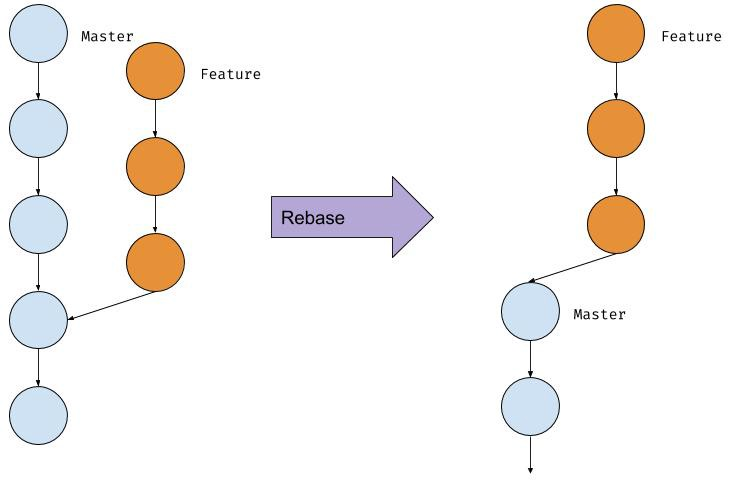
\includegraphics[width=0.4\linewidth]{pics/rebase-merge.jpeg}
    \vspace{-0.3cm}
    \caption{\footnotesize Regular architecture (Source: https://itnext.io)}
  \end{center}
\end{figure}
\item Interactive rebase to modify/delete commits
\comm{git rebase -i HEAD$\sim$3} (It starts editing the last 3 commits)
\end{enumerate}
\end{itemize}
\end{frame}
